% Funny bug http://tex.stackexchange.com/questions/232168/normal-text-is-invisible-when-using-beamer-with-notes-and-xelatex
\def\pgfsysdriver{pgfsys-dvipdfm.def}
\documentclass{beamer}
\title{Git Workshop}
\author{Peter Lundgren}

\usepackage{pgfpages}
\usepackage{ifthen}
\usepackage{pgfplots}
\pgfplotsset{compat=1.11}
\usepgfplotslibrary{dateplot}
\usepackage{adjustbox}
\usepackage{minibox}
\usepackage{subcaption}
\captionsetup{compatibility=false}
\usepackage{gitdags}
\usepackage{xcolor-solarized}
\usepackage{tikz}
\usetikzlibrary{fit,arrows,shadows}
\usepackage{hyperref}
\usepackage{multicol}
\usepackage{graphics}
\graphicspath{ {images/} }
\usepackage{enumitem}
% Don't let enumitem redefine beamer's template
\setitemize{label=\usebeamerfont*{itemize item}%
  \usebeamercolor[fg]{itemize item}
  \usebeamertemplate{itemize item}}
\usepackage{minted}

\makeatletter
% Courtesy of Section 102.5.3 of the Tikz & PGF Manual
\pgfdeclareshape{document}{
    \inheritsavedanchors[from=rectangle] % this is nearly a rectangle
    \inheritanchorborder[from=rectangle]
    \inheritanchor[from=rectangle]{center}
    \inheritanchor[from=rectangle]{north}
    \inheritanchor[from=rectangle]{south}
    \inheritanchor[from=rectangle]{west}
    \inheritanchor[from=rectangle]{east}
    % ... and possibly more
    \backgroundpath{% this is new
        % store lower right in xa/ya and upper right in xb/yb
        \southwest \pgf@xa=\pgf@x \pgf@ya=\pgf@y
        \northeast \pgf@xb=\pgf@x \pgf@yb=\pgf@y
        % compute corner of ‘‘flipped page’’
        \pgf@xc=\pgf@xb \advance\pgf@xc by-7.5pt % this should be a parameter
        \pgf@yc=\pgf@yb \advance\pgf@yc by-7.5pt
        % construct main path
        \pgfpathmoveto{\pgfpoint{\pgf@xa}{\pgf@ya}}
        \pgfpathlineto{\pgfpoint{\pgf@xa}{\pgf@yb}}
        \pgfpathlineto{\pgfpoint{\pgf@xc}{\pgf@yb}}
        \pgfpathlineto{\pgfpoint{\pgf@xb}{\pgf@yc}}
        \pgfpathlineto{\pgfpoint{\pgf@xb}{\pgf@ya}}
        \pgfpathclose
        % add little corner
        \pgfpathmoveto{\pgfpoint{\pgf@xc}{\pgf@yb}}
        \pgfpathlineto{\pgfpoint{\pgf@xc}{\pgf@yc}}
        \pgfpathlineto{\pgfpoint{\pgf@xb}{\pgf@yc}}
        \pgfpathlineto{\pgfpoint{\pgf@xc}{\pgf@yc}}
    }
}
\makeatother

\newcommand{\chapquote}[2]{
    \begin{quotation} {\itshape#1} \end{quotation}
    \begin{flushright} - #2 \end{flushright}
}

\AtBeginSection[]{
    \begin{frame}
    \frametitle{Table of Contents}
    \tableofcontents[currentsection]
    \end{frame}
}

\setbeamercolor{normal text}{fg=black}
\setbeamercolor{structure}{fg=solarized-blue,bg=solarized-base2!50}
\setbeamercolor{alerted text}{fg=solarized-orange}
\setbeamerfont{alerted text}{series=\bfseries}
\setbeamercolor{background canvas}{bg=solarized-base3!40}
\setbeamertemplate{background}{\tikz[overlay,remember picture]\node[] at (11.7, -8.5) {
\includegraphics[width=6em]{Git-Icon-base3.png}};}
\setbeameroption{show notes on second screen=right}
\setbeamertemplate{note page}[plain]
\setbeamertemplate{caption}[numbered]

% Fit multiple things on a slide closer together
\setlength\partopsep{-2\topsep}
\addtolength\partopsep{-2\parskip}

\begin{document}
    \begin{frame}
        \titlepage
    \end{frame}
    \note[itemize]{
        \item Introductions
        \item We've got a lot to talk about today
        \item We've also got a lot of time
        \item Ask questions
        \item Tell me if I'm going too fast
    }

    \begin{frame}
        \frametitle{More Information}
        \centering
        This presentation is avaliable at
        \url{https://github.com/peterlundgren/git-workshop}

        \bigskip
        Download Git at
        \url{https://git-scm.com}

        \bigskip
        Learn more about Git at
        \url{https://progit.org}
    \end{frame}

    \section[Section]{What is Git?}

\tikzset{
    box/.style={
        draw=solarized-base01,
        fill=solarized-base3!50,
        %thick,
        drop shadow={
            opacity=0.15,
        },
    },
    box2/.style={
        draw=solarized-base01,
        fill=solarized-base2!50,
        %thick,
        drop shadow={
            opacity=0.15,
        },
    },
    arrow/.style={
        %semithick,
        Latex-,
        draw=gray,
    },
    file/.style={
        shape=document,
        minimum height=4em,
        minimum width=3em,
        draw=solarized-base01,
        fill=solarized-blue!20,
        %thick,
        drop shadow={
            opacity=0.15,
        },
        font=\fontfamily{lmtt}\selectfont\small,
    },
    version/.style={
        shape=rounded rectangle,
        rounded rectangle arc length=90,
        minimum height=1.6em,
        minimum width=2em,
        draw=solarized-base01,
        fill=solarized-green!20,
        %very thick,
        drop shadow={
            opacity=0.15,
        },
        font=\fontfamily{lmtt}\selectfont\small,
    },
}

\newsavebox{\versiondatabase}
\savebox{\versiondatabase}{%
    \begin{tikzpicture}[node distance=1em]
        \pgfdeclarelayer{background}
        \pgfsetlayers{background,main}
        \node (vdb) [] {Version Database};
        \node (v3) [below=of vdb, version] {Version 3};
        \node (v2) [below=of v3, version] {Version 2};
        \node (v1) [below=of v2, version] {Version 1};
        \draw [arrow] (v2) -- (v3);
        \draw [arrow] (v1) -- (v2);
        \begin{pgfonlayer}{background}
            \node (vdbbox) [fit=(vdb)(v3)(v2)(v1),box2] {};
        \end{pgfonlayer}
    \end{tikzpicture}%
}

\newsavebox{\files}
\savebox{\files}{%
    \begin{tikzpicture}[]
        \foreach \i in {1,2,3} {
            \begin{scope}[shift={(.1*\i,.1*\i)}]
                \node () [file] {Files};
            \end{scope}
        }
    \end{tikzpicture}%
}

\begin{frame}
    \frametitle{What is Git?}
    \centering
    \minibox{
        git \textit{noun} \textbackslash'git\textbackslash\\
        \textit{British}\\
        \qquad : a foolish or worthless person
    }
\end{frame}

\begin{frame}
    \frametitle{What is Git?}
    Random three-letter combination that is pronounceable, and not actually
    used by any common UNIX command. The fact that it is a mispronunciation of
    "get" may or may not be relevant.
\end{frame}
\note{From the git README}

\begin{frame}
    \frametitle{What is Git?}
    \centering
    Git is an open source,\\
    distributed version control system\\
    designed for speed and efficiency
\end{frame}
\note{Official tagline of Git}

\begin{frame}
    \frametitle{What is Git?}
    \centering
    Git is an \alert{open source},\\
    distributed version control system\\
    designed for speed and efficiency
\end{frame}
\note[itemize]{
    \item LGPL-2.1
    \item https://github.com/git/git
}

\begin{frame}
    \frametitle{Linus Torvalds}
    \begin{columns}
        \begin{column}{0.38\textwidth}
            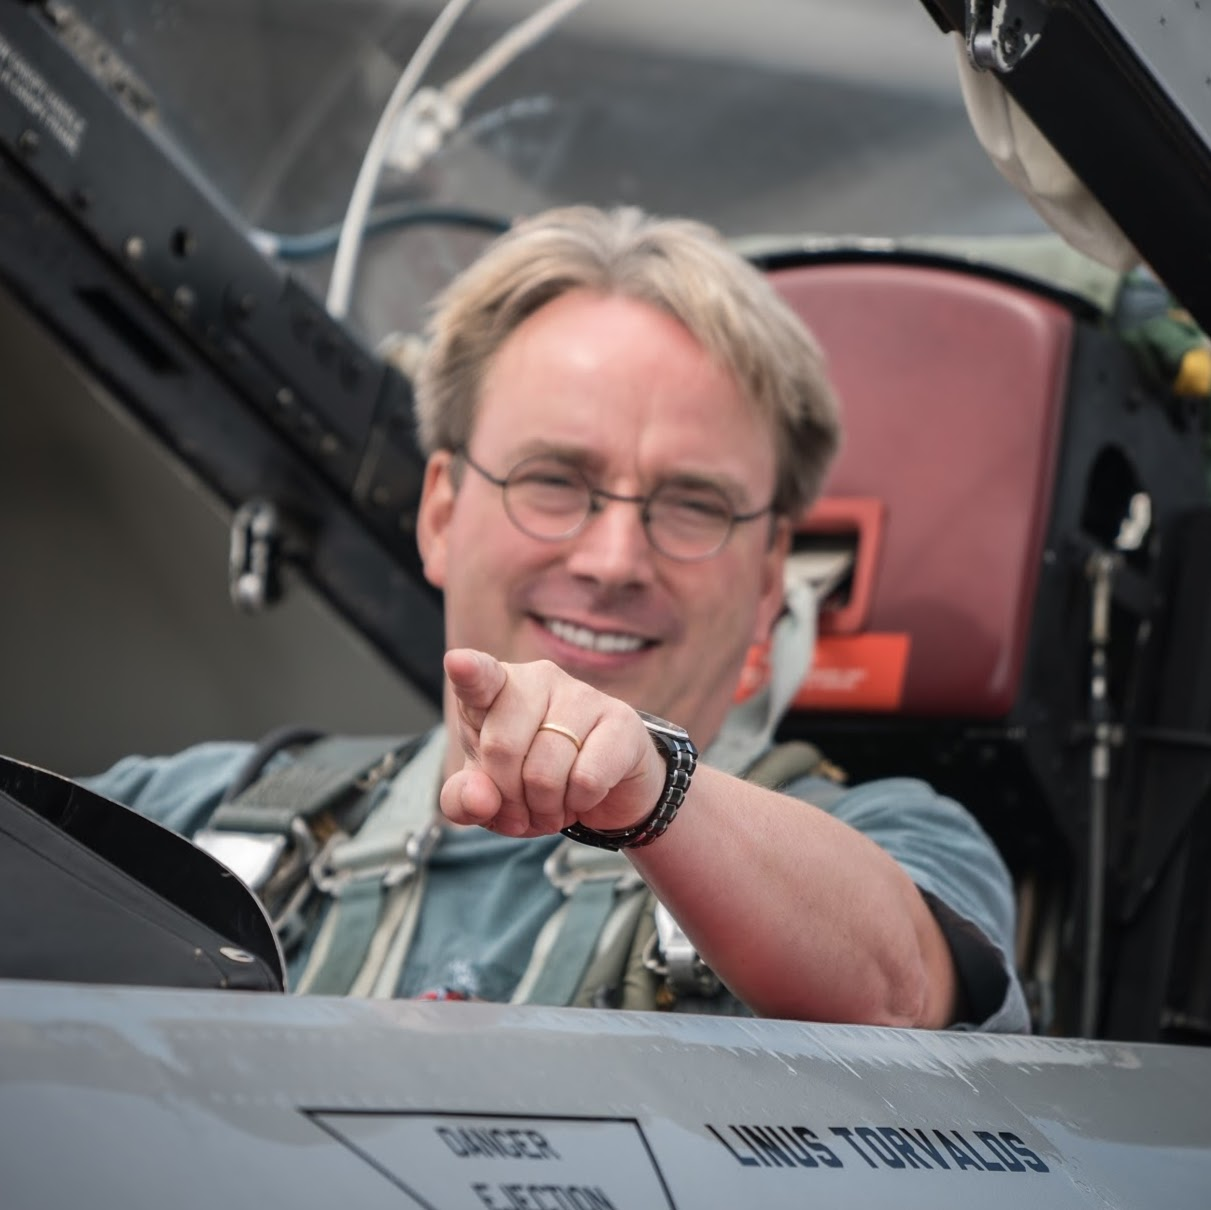
\includegraphics[width=1.2\textwidth]{Linus-Torvalds}
        \end{column}
        \begin{column}{0.62\textwidth}
            \chapquote{``I'm an egotistical bastard, and I name all my projects
                    after myself. First 'Linux', now 'Git'"}{Linus Torvalds}
        \end{column}
    \end{columns}
\end{frame}
\note[itemize]{
    \item First release was 7 April 2005 from Linus Torvalds
    \item Kernel hacker mentality. It was written to manage the Linux
          kernel. So, it won't stop you from shooting yourself in the foot.
}

\begin{frame}
    \frametitle{Junio Hamano}
    \centering
    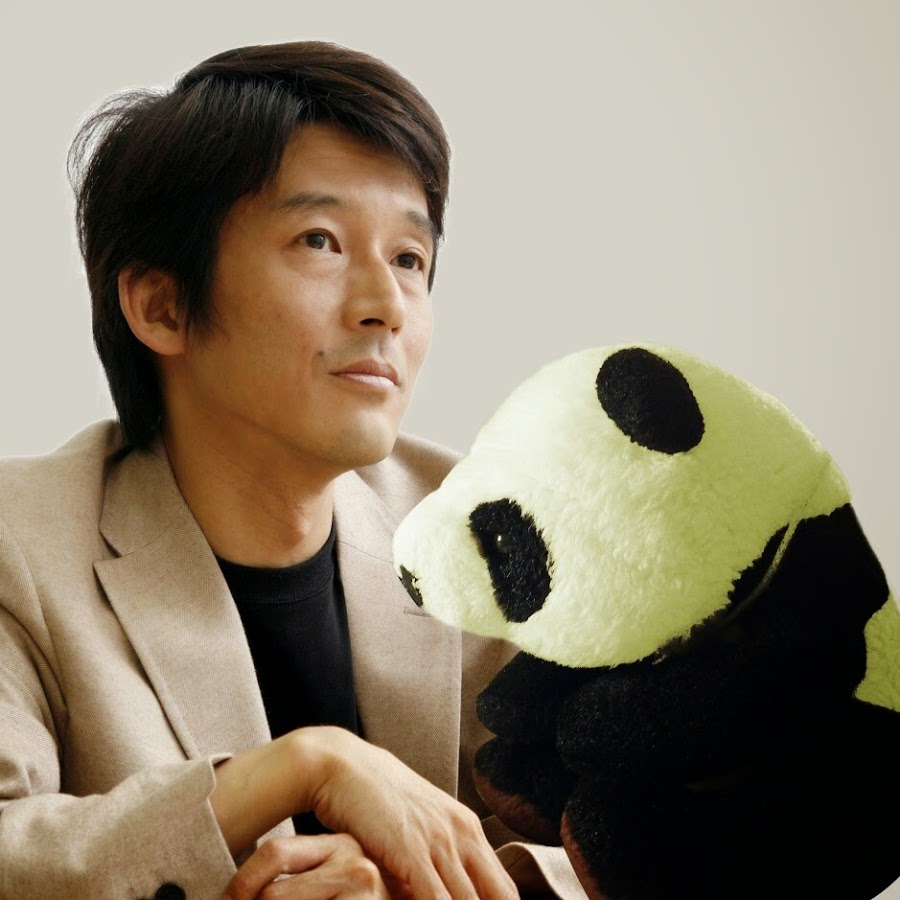
\includegraphics[width=\textwidth,height=0.8\textheight,keepaspectratio]{Junio-Hamano}
\end{frame}
\note[itemize]{
    \item Maintained by Junio Hamano since since 26 July 2005
}

\begin{frame}
    \frametitle{And Many More}
    {
        \fontsize{2.5}{4}\selectfont
        \setlength{\parskip}{3pt}
        \setlength{\parindent}{0pt}
        \setitemize[0]{leftmargin=*,rightmargin=0pt}
        \color{black}
        \setlength{\columnsep}{0pt}
        \begin{multicols}{7}
            \begin{itemize}
                \item[] Junio C Hamano
                \item[] Jeff King
                \item[] Shawn O. Pearce
                \item[] Linus Torvalds
                \item[] Nguyễn Thái Ngọc Duy
                \item[] Johannes Schindelin
                \item[] Michael Haggerty
                \item[] Jonathan Nieder
                \item[] René Scharfe
                \item[] Eric Wong
                \item[] Jakub Narębski
                \item[] Christian Couder
                \item[] Johannes Sixt
                \item[] Felipe Contreras
                \item[] Nicolas Pitre
                \item[] Paul Mackerras
                \item[] Thomas Rast
                \item[] Brandon Casey
                \item[] Ævar Arnfjörð Bjarmason
                \item[] Matthieu Moy
                \item[] Michael J Gruber
                \item[] Simon Hausmann
                \item[] Jiang Xin
                \item[] Petr Baudis
                \item[] Alex Riesen
                \item[] Stefan Beller
                \item[] Ramkumar Ramachandra
                \item[] Elia Pinto
                \item[] Eric Sunshine
                \item[] Johan Herland
                \item[] Miklos Vajna
                \item[] Ramsay Jones
                \item[] Daniel Barkalow
                \item[] J. Bruce Fields
                \item[] SZEDER Gábor
                \item[] David Aguilar
                \item[] John Keeping
                \item[] Pete Wyckoff
                \item[] Elijah Newren
                \item[] Kay Sievers
                \item[] Pierre Habouzit
                \item[] Jens Lehmann
                \item[] Stephen Boyd
                \item[] Tay Ray Chuan
                \item[] Ralf Thielow
                \item[] Paul Tan
                \item[] Alexandre Julliard
                \item[] Karsten Blees
                \item[] Martin von Zweigbergk
                \item[] Pat Thoyts
                \item[] Clemens Buchacher
                \item[] Giuseppe Bilotta
                \item[] Alexander Gavrilov
                \item[] Avery Pennarun
                \item[] Jay Soffian
                \item[] Torsten Bögershausen
                \item[] brian m. carlson
                \item[] Erik Faye-Lund
                \item[] Karthik Nayak
                \item[] Fredrik Kuivinen
                \item[] Nanako Shiraishi
                \item[] Ronnie Sahlberg
                \item[] Jim Meyering
                \item[] Frank Lichtenheld
                \item[] Jon Seymour
                \item[] Steffen Prohaska
                \item[] Brian Gernhardt
                \item[] Gerrit Pape
                \item[] Martin Langhoff
                \item[] Heiko Voigt
                \item[] Mike Hommey
                \item[] David Turner
                \item[] Vasco Almeida
                \item[] Peter Krefting
                \item[] Jonas Fonseca
                \item[] Markus Heidelberg
                \item[] Matthias Lederhofer
                \item[] Bert Wesarg
                \item[] Lars Hjemli
                \item[] Stephan Beyer
                \item[] Michele Ballabio
                \item[] Matthias Urlichs
                \item[] Kirill Smelkov
                \item[] Martin Koegler
                \item[] Nick Hengeveld
                \item[] Christian Stimming
                \item[] Andy Parkins
                \item[] Sergey Vlasov
                \item[] H. Peter Anvin
                \item[] Luben Tuikov
                \item[] Ryan Anderson
                \item[] Charles Bailey
                \item[] Mark Levedahl
                \item[] Sebastian Schuberth
                \item[] Luke Diamand
                \item[] Philip Oakley
                \item[] Thomas Ackermann
                \item[] Trần Ngọc Quân
                \item[] Ben Walton
                \item[] Lars Schneider
                \item[] Pavel Roskin
                \item[] Santi Béjar
                \item[] Adam Spiers
                \item[] Dmitry Potapov
                \item[] Marius Storm-Olsen
                \item[] Sverre Rabbelier
                \item[] Dan McGee
                \item[] Jon Loeliger
                \item[] Sean Estabrooks
                \item[] Sven Verdoolaege
                \item[] W. Trevor King
                \item[] Sam Vilain
                \item[] Björn Gustavsson
                \item[] Carlos Martín Nieto
                \item[] Uwe Kleine-König
                \item[] Aneesh Kumar K.V
                \item[] Lukas Sandström
                \item[] Matthew Ogilvie
                \item[] Han-Wen Nienhuys
                \item[] Michael G. Schwern
                \item[] Theodore Ts'o
                \item[] Wincent Colaiuta
                \item[] David Barr
                \item[] Michał Kiedrowicz
                \item[] Zbigniew Jędrzejewski-Szmek
                \item[] Andreas Ericsson
                \item[] Célestin Matte
                \item[] Patrick Steinhardt
                \item[] Dennis Stosberg
                \item[] Kyle J. McKay
                \item[] Tanay Abhra
                \item[] Alex Henrie
                \item[] Antoine Pelisse
                \item[] David Kastrup
                \item[] Jacob Keller
                \item[] Jean-Noel Avila
                \item[] Ralf Wildenhues
                \item[] Stefano Lattarini
                \item[] Julian Phillips
                \item[] Eric W. Biederman
                \item[] Ilari Liusvaara
                \item[] Martin Waitz
                \item[] Timo Hirvonen
                \item[] Yann Dirson
                \item[] Björn Steinbrink
                \item[] Kevin Ballard
                \item[] Richard Hansen
                \item[] Thomas Gummerer
                \item[] Carlos Rica
                \item[] Kjetil Barvik
                \item[] Kristian Høgsberg
                \item[] Max Kirillov
                \item[] Michael S. Tsirkin
                \item[] Paolo Bonzini
                \item[] Andy Whitcroft
                \item[] Jason Riedy
                \item[] Kevin Bracey
                \item[] Mark Lodato
                \item[] Michael Witten
                \item[] Robert Fitzsimons
                \item[] Robin Rosenberg
                \item[] Tim Henigan
                \item[] Alexander Shopov
                \item[] Dmitry Ivankov
                \item[] Karl Wiberg
                \item[] Peter Eriksen
                \item[] Brad King
                \item[] Josef Weidendorfer
                \item[] Matthias Kestenholz
                \item[] Vitor Antunes
                \item[] Adam Roben
                \item[] Anders Kaseorg
                \item[] Brian Downing
                \item[] Jari Aalto
                \item[] Lee Marlow
            \end{itemize}
        \end{multicols}
    }
\end{frame}
\note[itemize]{
    \item Just a few of Git's contributors
    \item 1430 Contributors listed as of 2016-08-30
}

\begin{frame}
    \frametitle{What is Git?}
    \centering
    Git is an open source,\\
    \alert{distributed} version control system\\
    designed for speed and efficiency
\end{frame}

\begin{frame}
    \frametitle{Centralized Version Control}
    \centering
    \begin{figure}
        \begin{tikzpicture}[node distance=1em]
            \pgfdeclarelayer{background}
            \pgfsetlayers{background,main}
            \node (server) [] {Server};
            \node (vdbbox) [below=of server,inner sep=0] {\usebox{\versiondatabase}};
            \node (client1) [] at (-4,-2) {Client A};
            \node (files1) [below=of client1,inner sep=0] {\usebox{\files}};
            \node (client2) [] at (4,-2) {Client B};
            \node (files2) [below=of client2,inner sep=0] {\usebox{\files}};
            \begin{pgfonlayer}{background}
                \node [fit=(server)(vdbbox),box] {};
                \node [fit=(client1)(files1),box] {};
                \node [fit=(client2)(files2),box] {};
            \end{pgfonlayer}
            \draw [arrow] (vdbbox) -- (files1);
            \draw [arrow] (files1) -- (vdbbox);
            \draw [arrow] (vdbbox) -- (files2);
            \draw [arrow] (files2) -- (vdbbox);
        \end{tikzpicture}
        \caption{Centralized Version Control}
    \end{figure}
\end{frame}
\note[itemize]{
    \item Client, server model
    \item Version database on only one server
    \item Download a snapshot
    \item Send incremental changes to the server
    \item Division of responsibility; some things only server can do, some
          things only client can do.
}

\begin{frame}
    \frametitle{Distributed Version Control}
    \begin{figure}
        \begin{adjustbox}{max totalsize={\textwidth}{\textheight},center}
            \begin{tikzpicture}[node distance=1.4em]
                \pgfdeclarelayer{background}
                \pgfsetlayers{background,main}
                \node (server) [] {Server};
                \node (vdbbox) [below=of server,inner sep=0] {\usebox{\versiondatabase}};
                \node (client1) [] at (-4,0) {Client A};
                \node (files1) [below=of client1,inner sep=0] {\usebox{\files}};
                \node (vdbbox1) [below=of files1,inner sep=0] {\usebox{\versiondatabase}};
                \node (client2) [] at (4,0) {Client B};
                \node (files2) [below=of client2,inner sep=0] {\usebox{\files}};
                \node (vdbbox2) [below=of files2,inner sep=0] {\usebox{\versiondatabase}};
                \begin{pgfonlayer}{background}
                    \node [fit=(server)(vdbbox),box] {};
                    \node [fit=(client1)(files1)(vdbbox1),box] {};
                    \node [fit=(client2)(files2)(vdbbox2),box] {};
                \end{pgfonlayer}
                \draw [arrow] (vdbbox) -- (vdbbox1);
                \draw [arrow] (vdbbox1) -- (vdbbox);
                \draw [arrow] (files1) -- (vdbbox1);
                \draw [arrow] (vdbbox1) -- (files1);
                \draw [arrow] (vdbbox) -- (vdbbox2);
                \draw [arrow] (vdbbox2) -- (vdbbox);
                \draw [arrow] (files2) -- (vdbbox2);
                \draw [arrow] (vdbbox2) -- (files2);
                \draw [arrow] ([yshift=-3em] vdbbox1.east) -- ([yshift=-3em] vdbbox2.west);
                \draw [arrow] ([yshift=-3em] vdbbox2.west) -- ([yshift=-3em] vdbbox1.east);
            \end{tikzpicture}
        \end{adjustbox}
        \caption{Distributed Version Control}
    \end{figure}
\end{frame}
\note[itemize]{
    \item Peer to peer
    \item Version database on every machine
    \item Clients can talk to each other
    \item Download the entire repository
    \item Operate locally, share explicitely
    \item You can have a central server
    \item Servers are only different in that, as an optimization, they
          don't have working copies of the files. The clients are actually
          more featureful than the server.
}

\begin{frame}
    \frametitle{What is Git?}
    \centering
    Git is an open source,\\
    distributed version control system\\
    designed for \alert{speed and efficiency}
\end{frame}

\newcommand{\gitsvnplot}[4]{%
    \begin{tikzpicture}[baseline]
        \ifthenelse{\equal{#1}{true}}{
            \begin{axis}[
                ybar=0,
                bar width=1.2cm,
                x=1.2cm,
                enlarge x limits={abs=0.1cm},
                ymin=0,
                symbolic x coords={#2},
                xtick=data,
                yticklabels={,,},
                tick style={draw=none},
                axis x line*=bottom,
                xticklabel style={
                    font=\small,
                },
                legend style={
                    %at={(1.5,1)},
                    fill=solarized-base3!40,
                    %draw=none,
                    draw=solarized-base01,
                },
                legend columns=-1,
                legend to name=foobar,
                legend entries={Git,Subversion},
                nodes near coords,
                nodes near coords={\pgfmathprintnumber[fixed,precision=2,zerofill=true]{\pgfplotspointmeta}},
                axis line style={solarized-base01},
                axis y line*=left,
                ylabel={Seconds},
                ylabel near ticks,
            ]
        }{
            \begin{axis}[
                ybar=0,
                bar width=1.2cm,
                x=1.2cm,
                enlarge x limits={abs=0.1cm},
                ymin=0,
                symbolic x coords={#2},
                xtick=data,
                yticklabels={,,},
                tick style={draw=none},
                axis x line*=bottom,
                xticklabel style={
                    font=\small,
                },
                legend style={
                    %at={(1.5,1)},
                    fill=solarized-base3!40,
                    %draw=none,
                    draw=solarized-base01,
                },
                legend columns=-1,
                legend to name=foobar,
                legend entries={Git,Subversion},
                nodes near coords,
                nodes near coords={\pgfmathprintnumber[fixed,precision=2,zerofill=true]{\pgfplotspointmeta}},
                scaled y ticks=false,
                axis line style={solarized-base01},
                hide y axis,
            ]
        }
            \addplot[solarized-orange,fill=solarized-orange!20] coordinates {(#2,#3)};
            \addplot[solarized-blue,fill=solarized-blue!20] coordinates {(#2,#4)};
        \end{axis}
    \end{tikzpicture}%
}
\begin{frame}
    \frametitle{Git is Fast}
    \begin{figure}
        \begin{adjustbox}{max totalsize={\textwidth}{.75\textheight},center}
            \begin{tabular}{llllll}
                \gitsvnplot{true}{Commit Files}{0.64}{2.60} &
                \gitsvnplot{false}{Commit Images}{1.53}{24.70} &
                \gitsvnplot{false}{Diff Current}{0.25}{1.09} &
                \gitsvnplot{false}{Diff Recent}{0.25}{3.99} &
                \gitsvnplot{false}{Diff Tags}{1.17}{83.57} &
                \gitsvnplot{false}{Clone}{107.5}{14.0} \\
                \gitsvnplot{true}{Log (50)}{0.01}{0.38} &
                \gitsvnplot{false}{Log (All)}{0.52}{169.20} &
                \gitsvnplot{false}{Log (File)}{0.60}{82.84} &
                \gitsvnplot{false}{Update}{0.90}{2.82} &
                \gitsvnplot{false}{Blame}{1.91}{3.04} &
                \gitsvnplot{false}{Size}{181.0}{132.0} \\
                \multicolumn{6}{r}{\ref{foobar}} \\
            \end{tabular}
        \end{adjustbox}
        \caption{Runtime of Git and Subversion Commands}
    \end{figure}
\end{frame}
\note[itemize]{
    \item Data from Scott Chacon http://git-scm.com/about/small-and-fast
    \item All operations are local except explicit synchronization
    \item No network access needed to:
    \begin{itemize}
        \item Perform a diff
        \item View file history
        \item Commit changes
        \item Merge branches
        \item Switch branches
        \item Checkout another revision
        \item Blame a file
        \item Search for the change that introduced a bug
    \end{itemize}
}

\begin{frame}
    \frametitle{What is Git?}
    \centering
    \alert{Immutable} \\
    (almost) never removes data
\end{frame}
\note[itemize]{
    \item You will hear about rewriting history.
    \item How many people have heard about rewriting history in Git?
    \item Git does not rewrite history.
    \item What Git does, is write a new history and move a pointer to it.
    \item Old history is still in the database.
    \item If you delete a branch, you're not deleting the work on that branch,
          you're deleting a pointer to it.
    \item Git keeps a log off all of this, so you can go back and find it.
}

\begin{frame}
    \frametitle{What is Git?}
    \centering
    Cryptographically \alert{secure}
\end{frame}
\note[itemize]{
    \item Everything is hashed and addressed by its hash.
    \item Change content, change how you get that content.
    \item Sign tags and commits with PGP.
    \item Git can detect corruption.
}

\begin{frame}
    \frametitle{Git is Popular}
    \centering
    % https://www.google.com/trends/explore?date=2005-05-01%202016-08-31&q=%2Fm%2F05vqwg,Subversion,%2Fm%2F08w6d6
    % Download csv in 4 year chunks to get weekly data
    % Adjust scale so that they match on overlapping weeks
    \begin{figure}
        \begin{tikzpicture}
            \begin{axis}[
                date coordinates in=x,
                xmin=2005-04-01,
                xmax=2016-09-01,
                ymin=0,
                ymax=226,
                width=\textwidth,
                height=0.8\textheight,
                yticklabels={,,},
                tick style={draw=none},
                xtick={2006-01-01,2008-01-01,2010-01-01,2012-01-01,2014-01-01,2016-01-01},
                xticklabel=\year,
                xticklabel style={
                    font=\scriptsize,
                },
                axis x line*=bottom,
                %hide y axis,
                axis y line*=left,
                axis line style={solarized-base01},
                legend style={
                    at={(0.6,1)},
                    fill=solarized-base3!40,
                    %draw=none,
                    draw=solarized-base01,
                    font=\scriptsize,
                },
                legend columns=-1,
            ]
                \addplot[solarized-orange] table [col sep=comma,x=Week,y=Git] {google-trends.csv};
                \addplot[solarized-blue] table [col sep=comma,x=Week,y=Subversion] {google-trends.csv};
                \addplot[solarized-violet] table [col sep=comma,x=Week,y=Perforce] {google-trends.csv};
                \legend{Git,Subversion,Perforce}
            \end{axis}
        \end{tikzpicture}
        \caption{Google Trends Since First Git Release}
    \end{figure}
\end{frame}
\note[itemize]{
    \item Dip every Christmas
}

    \section[Section]{Objectives}

\begin{frame}
\frametitle{Objectives}
\begin{itemize}
    \item Understand how Git works and how to apply that to day to day
          development
    \item Learn the basic 12 everyday commands
    \item Know how to undo mistakes
    \item Learn how to use Git to collaborate
    \item Learn how to find help
\end{itemize}
\end{frame}

\begin{frame}
\frametitle{12 Everyday Commands}
\begin{multicols}{3}
    \begin{itemize}
        \setlength\itemsep{3em}
        \item add
        \item branch
        \item checkout
        \item commit
        \item diff
        \item fetch
        \item help
        \item log
        \item merge
        \item push
        \item rebase
        \item status
    \end{itemize}
\end{multicols}
\end{frame}
\note[itemize]{
    \item Git has 160 subcommands in 2.9.3
    \item I'll cover about 20 of them
    \item These are the 12 you'll use daily
}

\begin{frame}
\frametitle{Finding Help}
\alert{Demo 01}: \texttt{git help}
\end{frame}
\note[itemize]{
    \item I'll cover one of them right now.
    \item Demo 01: git help
}

\begin{frame}
\frametitle{12 Everyday Commands}
\begin{multicols}{3}
    \begin{itemize}
        \setlength\itemsep{3em}
        \item add
        \item branch
        \item checkout
        \item commit
        \item diff
        \item fetch
        \item \alert{help}
        \item log
        \item merge
        \item push
        \item rebase
        \item status
    \end{itemize}
\end{multicols}
\end{frame}
\note[itemize]{
    \item One down, 11 to go.
}

\begin{frame}
\frametitle{Learn 4 Ways}
\begin{itemize}
    \setlength\itemsep{3em}
    \item Conceptual
    \item Commands
    \item Implementation
    \item Try It
\end{itemize}
\end{frame}
\note[itemize]{
    \item Conceptual - Computer science lecture. Diagrams of directed acyclic
          graphs and reachability. I'll lecture. We'll watch some lectures from
          Scott Chacon (Author of "Pro Git", CIO GitHub).
    \item Commands - Practical. How to use common commands.
    \item Implementation - How Git works under the hood.
    \item Try It - Practice!
}

    \section[Section]{Your First Repository}

\begin{frame}
    \frametitle{Your First Repository}
    \alert{Demo 2}: \texttt{git init}
\end{frame}
\note[itemize]{
    \item \alert{Demo 2}: \texttt{git init}
}

    \section[Section]{Three Stage Thinking}

\begin{frame}
    \frametitle{Three Stage Thinking}
    \begin{itemize}
        \setlength\itemsep{3em}
        \item Edit
        \item Add
        \item Commit
    \end{itemize}
\end{frame}

\begin{frame}
    \frametitle{Three Stage Thinking}
    \alert{Demo 03}: Three Stage Thinking
\end{frame}
\note[itemize]{
    \item Demo 03: Three Stage Thinking
}

\begin{frame}
    \frametitle{Lesson 1}
    \alert{Lesson 1}: Three Stage Thinking
\end{frame}

\begin{frame}
    \frametitle{12 Everyday Commands}
    \begin{multicols}{3}
        \begin{itemize}
            \setlength\itemsep{3em}
            \item \alert{add}
            \item branch
            \item checkout
            \item \alert{commit}
            \item \alert{diff}
            \item fetch
            \item \alert{help}
            \item \alert{log}
            \item merge
            \item push
            \item rebase
            \item \alert{status}
        \end{itemize}
    \end{multicols}
\end{frame}
\note[itemize]{
    \item You've already seen these
}

    \section[Section]{Trees, Hashes, and Blobs}

\begin{frame}
    \frametitle{Trees, Hashes, and Blobs}
    \alert{oh My!}
\end{frame}
\note[itemize]{
    \item \url{http://youtu.be/ZDR433b0HJY?t=13m17s} - 0:21:02
}

\begin{frame}
    \frametitle{Trees, Hashes, and Blobs}
    \alert{Demo 4}: Trees, Hashes, and Blobs
\end{frame}
\note[itemize]{
    \item \alert{Demo 4}: Trees, Hashes, and Blobs
}

    \section[Section]{Branch and Merge}

{
% Fit multiple things on a slide closer together
\setlength\partopsep{-2\topsep}

\begin{frame}
    \frametitle{Branch and Merge}
    \alert{Video}
\end{frame}
\note[itemize]{
    \item \alert{Video}: \url{http://youtu.be/ZDR433b0HJY?t=21m05s} - 0:30:35
}

\begin{frame}
    \frametitle{Branches}
    \centering
    \begin{figure}
        \begin{tikzpicture}
            \gitDAG[grow right sep=2em]{
                A
            };
            \gitbranch{master}{above=of A}{A}
        \end{tikzpicture}
        \caption{Branches are Pointers to Commits}
    \end{figure}
\end{frame}
\note[itemize]{
    \item By default, `git init` will create a master branch
    \item Most repositories have a master branch because most people are too
          lazy to change defaults
    \item Branches are pointers that point to commits
}

\begin{frame}
    \frametitle{\texttt{HEAD}}
    \centering
    \begin{figure}
        \begin{tikzpicture}
            \gitDAG[grow right sep=2em]{
                A
            };
            \gitbranch{master}{above=of A}{A}
            \gitHEAD{above=of master}{master}
        \end{tikzpicture}
        \caption{\texttt{HEAD} Points to Your Current Branch}
    \end{figure}
\end{frame}
\note[itemize]{
    \item \texttt{HEAD} points to current branch
    \item \texttt{HEAD} is what you have checked out on your filesytem
    \item \texttt{HEAD} is the parent of your next commit
}

\begin{frame}[fragile]
    \frametitle{\texttt{git branch}}
    \centering
    \begin{figure}
        \begin{tikzpicture}
            \gitDAG[grow right sep=2em]{
                A
            };
            \gitbranch{master}{above=of A}{A}
            \gitHEAD{above=of master}{master}
            \gitbranch{foo}{below=of A}{A}
        \end{tikzpicture}
        \caption{Creating a New Branch}
    \end{figure}
    \begin{minted}[bgcolor=solarized-base2!50,frame=single,framesep=3pt]{console}
$ git branch foo
    \end{minted}
\end{frame}
\note[itemize]{
    \item \texttt{HEAD} points to current branch
    \item \texttt{HEAD} is what you have checked out on your filesytem
    \item \texttt{HEAD} is the parent of your next commit
    \item Branches are cheap and fast. Writes 41 bytes to a file; that's it.
    \item \texttt{git branch foo} Creates a new branch called foo pointing to
          the same commit that HEAD is pointing to.
}

\begin{frame}[fragile]
    \frametitle{\texttt{git checkout}}
    \centering
    \begin{figure}
        \begin{tikzpicture}
            \gitDAG[grow right sep=2em]{
                A
            };
            \gitbranch{master}{above=of A}{A}
            \oldgitHEAD{above=of master}{master}
            \gitbranch{foo}{below=of A}{A}
            \gitHEAD{below=of foo}{foo}
        \end{tikzpicture}
        \caption{Switching Branches}
    \end{figure}
    \begin{minted}[bgcolor=solarized-base2!50,frame=single,framesep=3pt]{console}
$ git checkout foo
$ git branch
* foo
  master
    \end{minted}
\end{frame}
\note[itemize]{
    \item \texttt{git checkout} switches the current branch by changing what
          \texttt{HEAD} points to. If necessary, it will update your
          filesystem to match the commit pointed to by the branch.
    \item \texttt{git branch} will show you all of the local branches and put a
          star next to your current branch.
}

\begin{frame}[fragile]
    \frametitle{Make a Commit}
    \centering
    \begin{figure}
        \begin{tikzpicture}
            \gitDAG[grow right sep=2em]{
                A -- B
            };
            \gitbranch{master}{above=of A}{A}
            \oldgitbranch{foo}{below=of A}{A}
            \oldgitHEAD{below=of foo}{foo}
            \gitbranch{foo}{below=of B}{B}
            \gitHEAD{below=of foo}{foo}
        \end{tikzpicture}
        \caption{Make a Commit}
    \end{figure}
    \begin{minted}[bgcolor=solarized-base2!50,frame=single,framesep=3pt]{console}
$ git commit
    \end{minted}
\end{frame}
\note[itemize]{
    \item \texttt{git commit} Creates a new commit who's parent is whatever
          commit HEAD is pointing at. Then, it moves the branch \texttt{HEAD}
          is pointing at to the new commit.
    \item The only branch that moves is what \texttt{HEAD} points at.
    \item If you're ever scared about doing something, drop a branch behind. As
          long as you don't have a branch checked out, it's impossible to lose
          where it was.
}

\begin{frame}[fragile]
    \frametitle{Make Another Commit}
    \centering
    \begin{figure}
        \begin{tikzpicture}
            \gitDAG[grow right sep=2em]{
                A -- B -- C
            };
            \gitbranch{master}{above=of A}{A}
            \oldgitbranch{foo}{below=of B}{B}
            \oldgitHEAD{below=of foo}{foo}
            \gitbranch{foo}{below=of C}{C}
            \gitHEAD{below=of foo}{foo}
        \end{tikzpicture}
        \caption{Make Another Commit}
    \end{figure}
    \begin{minted}[bgcolor=solarized-base2!50,frame=single,framesep=3pt]{console}
$ git commit
    \end{minted}
\end{frame}

\begin{frame}[fragile]
    \frametitle{Checkout a New Branch}
    \centering
    \begin{figure}
        \begin{tikzpicture}
            \gitDAG[grow right sep=2em]{
                A -- B -- C
            };
            \gitbranch{master}{above=of A}{A}
            \gitbranch{bar}{below=of A}{A}
            \gitHEAD{below=of bar}{bar}
            \gitbranch{foo}{below=of C}{C}
            \oldgitHEAD{below=of foo}{foo}
        \end{tikzpicture}
        \caption{Checkout a New Branch}
    \end{figure}
    \begin{minted}[bgcolor=solarized-base2!50,frame=single,framesep=3pt]{console}
$ git checkout -b bar master
    \end{minted}
\end{frame}
\note[itemize]{
    \item \texttt{git checkout -b} is a shortcut for creating a branch and
          immediately checking it out.
}

\begin{frame}[fragile]
    \frametitle{Work on a New Branch}
    \centering
    \begin{figure}
        \begin{tikzpicture}
            \gitDAG[grow right sep=2em]{
                A -- {D -- E, B -- C}
            };
            \gitbranch{master}{above=of A}{A}
            \gitbranch{foo}{below=of C}{C}
            \gitbranch{bar}{above=of E}{E}
            \gitHEAD{above=of bar}{bar}
            \oldgitbranch{bar}{below=of A}{A}
            \oldgitHEAD{below=of bar}{bar}
        \end{tikzpicture}
        \caption{Work on a New Branch}
    \end{figure}
    \begin{minted}[bgcolor=solarized-base2!50,frame=single,framesep=3pt]{console}
$ git commit
$ git commit
    \end{minted}
\end{frame}
\note[itemize]{
    \item Make two commits on branch bar
}

\begin{frame}[fragile]
    \frametitle{Merging}
    \centering
    \begin{figure}
        \begin{tikzpicture}
            \gitDAG[grow right sep=2em]{
                A -- {D -- E, B -- C}
            };
            \gitbranch{master}{above=of A}{A}
            \gitbranch{foo}{below=of C}{C}
            \gitbranch{bar}{above=of E}{E}
            \gitHEAD{above=of master}{master}
            \oldgitHEAD{above=of bar}{bar}
        \end{tikzpicture}
        \caption{Checkout master}
    \end{figure}
    \begin{minted}[bgcolor=solarized-base2!50,frame=single,framesep=3pt]{console}
$ git checkout master
    \end{minted}
\end{frame}
\note[itemize]{
    \item Checkout the branch you want to modify / merge into
    \item Switch back to the master branch
    \item Next, I want the master have the changes on the bar branch
    \item \alert{Question}: What should happen?
    \item Git checks to see if master is reachable from bar. If it is, it does
          the easiest possible thing.
}

\begin{frame}[fragile]
    \frametitle{Fast-Forward Merge}
    \centering
    \begin{figure}
        \begin{tikzpicture}
            \gitDAG[grow right sep=2em]{
                A -- {D -- E, B -- C}
            };
            \gitbranch{master}{above left=of E}{E}
            \gitbranch{foo}{below=of C}{C}
            \gitbranch{bar}{above=of E}{E}
            \gitHEAD{above=of master}{master}
            \oldgitbranch{master}{above=of A}{A}
            \oldgitHEAD{above=of master}{master}
        \end{tikzpicture}
        \caption{Fast-Forward Merge}
    \end{figure}
    \begin{minted}[bgcolor=solarized-base2!50,frame=single,framesep=3pt]{console}
$ git merge bar
    \end{minted}
\end{frame}
\note[itemize]{
    \item Want master took look like bar.
    \item It moves master up to the same commit that bar is at.
    \item Next, merge foo.
    \item \alert{Question}: What should happen?
    \item It's going to do a non-fast-forward merge. It has to create a new
          tree. The snapshot with both master and foo doesn't exist yet.
}

\begin{frame}[fragile]
    \frametitle{Non-Fast-Forward Merge}
    \centering
    \begin{figure}
        \begin{tikzpicture}
            \gitDAG[grow right sep=2em]{
                A -- {D -- E, B -- C} -- F
            };
            \gitbranch{master}{above=of F}{F}
            \gitbranch{foo}{below=of C}{C}
            \gitbranch{bar}{above=of E}{E}
            \gitHEAD{above=of master}{master}
            \oldgitbranch{master}{above left=of E}{E}
            \oldgitHEAD{above=of master}{master}
        \end{tikzpicture}
        \caption{Non-Fast-Forward Merge}
    \end{figure}
    \begin{minted}[bgcolor=solarized-base2!50,frame=single,framesep=3pt]{console}
$ git merge foo
    \end{minted}
\end{frame}
\note[itemize]{
    \item Git created a new snapshot, F, and moved master to it.
    \item F now has both the changes on foo and bar.
    \item Git encodes this by having a commit with two parents.
    \item Neither foo nor bar moved. Branches that are not checked out will not
          move.
}

\begin{frame}
    \frametitle{Lesson 2}
    \alert{Lesson 2}: Branching and Merging
\end{frame}
\note[itemize]{
    \item \alert{Lesson 2}: Branching and Merging
    \item Demo lesson afterwards.
    \item cat .git/HEAD
    \item cat .git/refs/heads/feature/change-name
    \item Branches are just 41 byte files.
}

\begin{frame}
    \frametitle{Tags}
    Branches that Don't Move
\end{frame}
\note[itemize]{
    \item If you understand branches, then tags are easy.
}

\begin{frame}
    \frametitle{Lesson 3}
    \alert{Lesson 3}: Tags
\end{frame}
\note[itemize]{
    \item \alert{Lesson 3}: Tags
    \item Start discussion: Lightweight vs. annotated tags.
}

\begin{frame}
    \frametitle{12 Everyday Commands}
    \begin{multicols}{3}
        \begin{itemize}
            \setlength\itemsep{3em}
            \item \alert{add}
            \item \alert{branch}
            \item \alert{checkout}
            \item \alert{commit}
            \item \alert{diff}
            \item fetch
            \item \alert{help}
            \item \alert{log}
            \item \alert{merge}
            \item push
            \item rebase
            \item \alert{status}
        \end{itemize}
    \end{multicols}
\end{frame}
\note[itemize]{
    \item We've added branch, checkout, and merge
}

}

    \section[Section]{Rebase}

{
% Fit multiple things on a slide closer together
\setlength\partopsep{-2\topsep}

\begin{frame}
    \frametitle{Rebase}
    \centering
    With great power comes great responsibility
\end{frame}
\note[itemize]{
    \item Swiss-army-knife of rewriting history
    \item The ability to edit or rewrite history sets Git apart from other
          version control systems
}

{
\setbeamertemplate{background}{}
\setbeamertemplate{background}{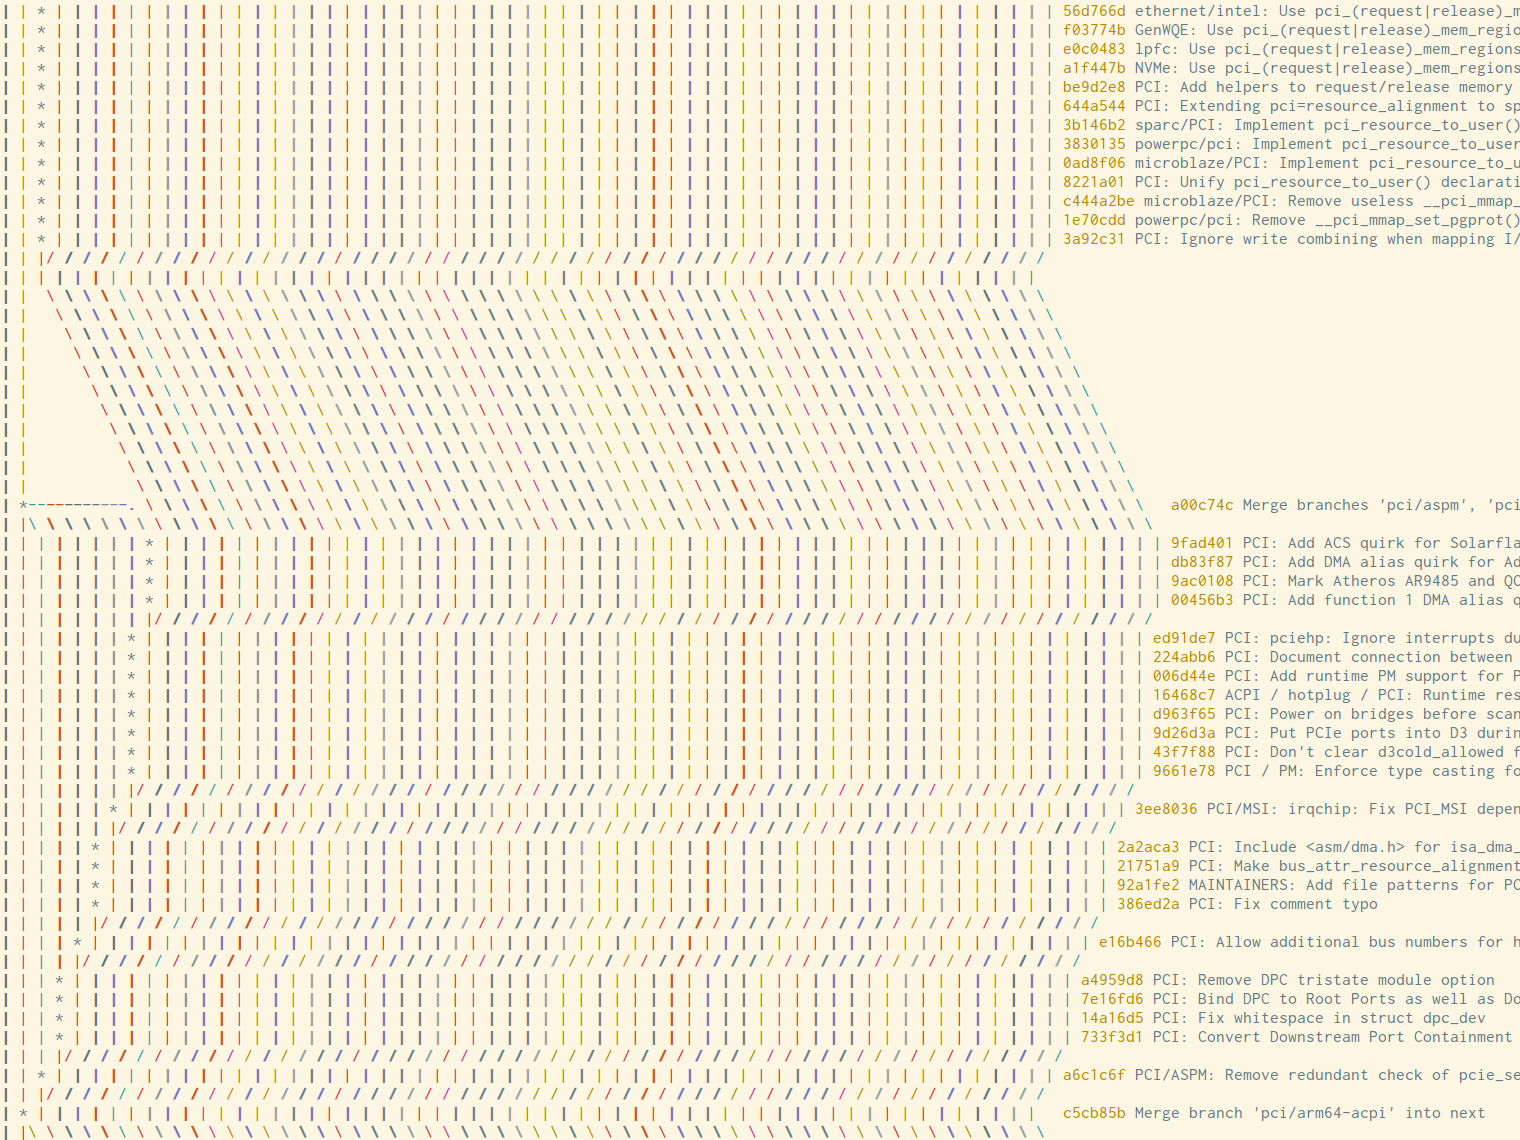
\includegraphics[width=\paperwidth]{images/linux-branches.png}}
\begin{frame}[plain]
\end{frame}
\note[itemize]{
    \item Long running branches can be confusing
    \item This is from the linux kernel
}
}

\begin{frame}
    \frametitle{Developing in Parallel or Taking Turns}
    \begin{figure}
        \begin{subfigure}[b]{\textwidth}
            \centering
            \begin{tikzpicture}
                \gitDAG[grow right sep=2em]{
                    A -- {{B, C -- D} -- H, E -- F -- G} -- I
                };
            \end{tikzpicture}
            \subcaption{Multiple Concurrent Branches}
        \end{subfigure}
        \begin{subfigure}[b]{\textwidth}
            \centering
            \begin{tikzpicture}
                \gitDAG[grow right sep=2em]{
                    A -- B -- C -- D -- E -- F -- G
                };
            \end{tikzpicture}
            \subcaption{Linear History}
        \end{subfigure}
        \caption{Two Ways to Tell a Story}
    \end{figure}
\end{frame}
\note[itemize]{
    \item What if we could use our version control tool to pretend that we took
          turns even when we develop in parallel
    \item Edit the top history to look like the bottom
    \item Is this even a good idea?
    \item The first use of \texttt{git rebase} we will look at will do this
}

\begin{frame}
    \frametitle{Rebase}
    \begin{figure}
        \centering
        \begin{tikzpicture}
            \gitDAG[grow right sep=2em]{
                A -- {{B, C -- D} -- {[nodes=unreachable] H},
                E -- F -- G} -- {[nodes=unreachable] I}
            };
            \gitbranch{master}{above=of B}{B}
            \gitHEAD{above=of master}{master}
            \gitbranch{foo}{right=of D}{D}
            \gitbranch{bar}{right=of G}{G}
        \end{tikzpicture}
        \caption{Two Branches to Rebase}
    \end{figure}
\end{frame}
\note[itemize]{
    \item Instead of creating the merge commits H and I we'll rebase foo and
          bar onto master in order to create a linear history
}

\begin{frame}[fragile]
    \frametitle{Rebase}
    \begin{figure}
        \centering
        \begin{tikzpicture}
            \gitDAG[grow right sep=2em]{
                A -- {{B, C -- D},
                E -- F -- G}
            };
            \gitbranch{master}{above=of B}{B}
            \oldgitHEAD{above=of master}{master}
            \gitbranch{foo}{right=of D}{D}
            \gitHEAD{right=of foo}{foo}
            \gitbranch{bar}{right=of G}{G}
        \end{tikzpicture}
        \caption{Checkout foo}
    \end{figure}
    \begin{minted}[bgcolor=solarized-base2!50,frame=single,framesep=3pt]{console}
$ git checkout foo
    \end{minted}
\end{frame}
\note[itemize]{
    \item First, we'll rebase foo onto master
    \item We must checkout foo first
    \item Remember Git will not touch branches you don't have checked out
    \item We want to take the branch foo, containing commits C and D, and
          reaply them after commit B
}

\begin{frame}[fragile]
    \frametitle{Rebase}
    \begin{figure}
        \centering
        \begin{tikzpicture}
            \gitDAG[grow right sep=2em]{
                A -- {{B -- C' -- D', {[nodes=unreachable] C -- D}},
                E -- F -- G}
            };
            \gitbranch{master}{above=of B}{B}
            \oldgitbranch{foo}{right=of D}{D}
            \oldgitHEAD{right=of foo}{foo}
            \gitbranch{foo}{above=of D'}{D'}
            \gitHEAD{above=of foo}{foo}
            \gitbranch{bar}{right=of G}{G}
        \end{tikzpicture}
        \caption{Rebase foo onto master}
    \end{figure}
    \begin{minted}[bgcolor=solarized-base2!50,frame=single,framesep=3pt]{console}
$ git rebase master
    \end{minted}
\end{frame}
\note[itemize]{
    \item ... to do that, we use the command \texttt{git rebase master}
    \item Commits C' and D' have the
    \begin{itemize}
        \item same deltas as C and D,
        \item same commit message,
        \item same author,
    \end{itemize}
    \item but different sha1sum because they have
    \begin{itemize}
        \item different parents,
        \item and different trees (different snapshots);
        \item because the snapshots also contain the changes in B
    \end{itemize}
    \item Rebase works by
    \begin{itemize}
        \item first finding a common ancestor (A)
        \item making patches for each commit in the source branch
        \item and reapplying them on the destination branch
    \end{itemize}
}

\begin{frame}[fragile]
    \frametitle{Rebase}
    \begin{figure}
        \centering
        \begin{tikzpicture}
            \gitDAG[grow right sep=2em]{
                A -- {{B -- C' -- D', {[nodes=placeholder] C -- D}},
                E -- F -- G}
            };
            \gitbranch{master}{above=of B}{B}
            \gitbranch{foo}{above=of D'}{D'}
            \oldgitHEAD{above=of foo}{foo}
            \gitbranch{bar}{right=of G}{G}
            \gitHEAD{above=of bar}{bar}
        \end{tikzpicture}
        \caption{Checkout bar}
    \end{figure}
    \begin{minted}[bgcolor=solarized-base2!50,frame=single,framesep=3pt]{console}
$ git checkout bar
    \end{minted}
\end{frame}
\note[itemize]{
    \item Repeat the process for branch bar
}

\begin{frame}[fragile]
    \frametitle{Rebase}
    \begin{figure}
        \centering
        \begin{tikzpicture}
            \gitDAG[grow right sep=2em]{
                A -- {{B -- C' -- D' -- E' -- F' -- G',
                {[nodes=placeholder] C -- D}},
                {[nodes=unreachable] E -- F -- G}}
            };
            \gitbranch{master}{above=of B}{B}
            \gitbranch{foo}{above=of D'}{D'}
            \oldgitbranch{bar}{right=of G}{G}
            \oldgitHEAD{above=of bar}{bar}
            \gitbranch{bar}{above=of G'}{G'}
            \gitHEAD{above=of bar}{bar}
        \end{tikzpicture}
        \caption{Rebase bar Onto foo}
    \end{figure}
    \begin{minted}[bgcolor=solarized-base2!50,frame=single,framesep=3pt]{console}
$ git rebase foo
    \end{minted}
\end{frame}
\note[itemize]{
    \item Reapply E, F, and G after D'
}

\begin{frame}[fragile]
    \frametitle{Rebase}
    \begin{figure}
        \centering
        \begin{tikzpicture}
            \gitDAG[grow right sep=2em]{
                A -- B -- C' -- D' -- E' -- F' -- G'
            };
            \gitbranch{master}{above=of B}{B}
            \gitHEAD{above=of master}{master}
            \gitbranch{foo}{above=of D'}{D'}
            \gitbranch{bar}{above=of G'}{G'}
            \oldgitHEAD{above=of bar}{bar}
        \end{tikzpicture}
        \caption{Update master}
    \end{figure}
    \begin{minted}[bgcolor=solarized-base2!50,frame=single,framesep=3pt]{console}
$ git checkout master
    \end{minted}
\end{frame}
\note[itemize]{
    \item Now that we have the version of history that we want, let's update
          master
    \item First checkout master
}

\begin{frame}[fragile]
    \frametitle{Rebase}
    \begin{figure}
        \centering
        \begin{tikzpicture}
            \gitDAG[grow right sep=2em]{
                A -- B -- C' -- D' -- E' -- F' -- G'
            };
            \oldgitbranch{master}{above=of B}{B}
            \oldgitHEAD{above=of master}{master}
            \gitbranch{foo}{above=of D'}{D'}
            \gitbranch{bar}{above left=of G'}{G'}
            \gitbranch{master}{above=of G'}{G'}
            \gitHEAD{above=of master}{master}
        \end{tikzpicture}
        \caption{Merge Changes Into master}
    \end{figure}
    \begin{minted}[bgcolor=solarized-base2!50,frame=single,framesep=3pt]{console}
$ git merge bar
    \end{minted}
\end{frame}
\note[itemize]{
    \item Merge bar into master
    \item What kind of merge is this? Fast-forward merge
}

\begin{frame}[fragile]
    \frametitle{Rebase}
    \begin{figure}
        \centering
        \begin{tikzpicture}
            \gitDAG[grow right sep=2em]{
                A -- B -- C' -- D' -- E' -- F' -- G'
            };
            \oldgitbranch{foo}{above=of D'}{D'}
            \oldgitbranch{bar}{above left=of G'}{G'}
            \gitbranch{master}{above=of G'}{G'}
            \gitHEAD{above=of master}{master}
        \end{tikzpicture}
        \caption{Delete Branches}
    \end{figure}
    \begin{minted}[bgcolor=solarized-base2!50,frame=single,framesep=3pt]{console}
$ git branch -d foo
$ git branch -d bar
    \end{minted}
\end{frame}
\note[itemize]{
    \item If foo and bar are not needed anymore
}

\begin{frame}
    \frametitle{Lesson 4}
    \alert{Lesson 4}: Rebase
\end{frame}
\note[itemize]{
    \item \alert{Lesson 4}: Rebase
}

\begin{frame}
    \frametitle{Merge vs. Rebase}
    \begin{figure}
        \begin{subfigure}[b]{\textwidth}
            \centering
            \begin{tikzpicture}
                \gitDAG[grow right sep=2em]{
                    A -- {{B, C -- D} -- H, E -- F -- G} -- I
                };
            \end{tikzpicture}
            \subcaption{Multiple Concurrent Branches}
        \end{subfigure}
        \begin{subfigure}[b]{\textwidth}
            \centering
            \begin{tikzpicture}
                \gitDAG[grow right sep=2em]{
                    A -- B -- C' -- D' -- E' -- F' -- G'
                };
            \end{tikzpicture}
            \subcaption{Linear History}
        \end{subfigure}
        \caption{Two Ways to Tell a Story}
    \end{figure}
\end{frame}
\note[itemize]{
    \item Two ways to apply your changes to the mainline
    \item Start discussion: Merge vs. Rebase
}

\begin{frame}
    \frametitle{Interactive Rebase}
    \alert{Demo 5}: \texttt{git rebase --interactive}
\end{frame}
\note[itemize]{
    \item \alert{Demo 5}: \texttt{git rebase --interactive}
    \item Reorder, add, remove, edit, reword, squash commits
}

\begin{frame}
    \frametitle{Lesson 5}
    \alert{Lesson 5}: Interactive Rebase
\end{frame}
\note[itemize]{
    \item \alert{Lesson 5}: Interactive Rebase
}

\begin{frame}
    \frametitle{12 Everyday Commands}
    \begin{multicols}{3}
        \begin{itemize}
            \setlength\itemsep{3em}
            \item \alert{add}
            \item \alert{branch}
            \item \alert{checkout}
            \item \alert{commit}
            \item \alert{diff}
            \item fetch
            \item \alert{help}
            \item \alert{log}
            \item \alert{merge}
            \item push
            \item \alert{rebase}
            \item \alert{status}
        \end{itemize}
    \end{multicols}
\end{frame}
\note[itemize]{
    \item Now we've learned rebase
}

}

\end{document}
